\documentclass[10pt,a4paper]{article}
\usepackage{enumerate}
\usepackage{courier}
\usepackage{graphicx}
% \usepackage{tabularx}
% \usepackage{longtable}
%^ using xltabular instead as it includes the capabilities of both of the above
\usepackage{xltabular}
\usepackage[export]{adjustbox}
\usepackage{float}
\usepackage[utf8]{inputenc}
\usepackage[english]{babel}
\usepackage[english]{isodate}
\usepackage[parfill]{parskip}
\usepackage[margin=1.1in]{geometry}
\usepackage[titletoc,title]{appendix}
\usepackage{caption}
\usepackage{listings}
\usepackage{url}
\usepackage{pbox}
\usepackage{makecell}
\usepackage[T1]{fontenc}

\captionsetup{justification=raggedright, singlelinecheck=false}

% Fix for weird errors when quotes are in a string
\let\textquotedbl=" 

\newenvironment{spaceditemize}
{ \begin{itemize}
    \setlength{\itemsep}{5pt}
    \setlength{\parskip}{0pt}
    \setlength{\parsep}{0pt}     }
{ \end{itemize}                  } 

\newenvironment{spacedenumerate}
{ \begin{enumerate}
    \setlength{\itemsep}{5pt}
    \setlength{\parskip}{0pt}
    \setlength{\parsep}{0pt}     }
{ \end{enumerate}                } 

%%%%%%%%%%%%%%%%%%%%%%%%
% Commandline stuff
%%%%%%%%%%%%%%%%%%%%%%%
\usepackage{color}

\lstset{frame=leftline,
  aboveskip=3mm,
  belowskip=3mm,
  showstringspaces=false,
  columns=flexible,
  basicstyle={\small\ttfamily},
  numbers=none,
  breaklines=true,
  breakatwhitespace=true,
  tabsize=2
}

%%%%%%%%%%%%%%%%%%%%%%%%
% YAML stuff
%%%%%%%%%%%%%%%%%%%%%%%%
\usepackage[dvipsnames]{xcolor}

\newcommand\YAMLcolonstyle{\color{black}\mdseries\small}
\newcommand\YAMLkeystyle{\color{black}\bfseries\ttfamily\small}
\newcommand\YAMLvaluestyle{\color{black}\mdseries\small}

\makeatletter

% here is a macro expanding to the name of the language
% (handy if you decide to change it further down the road)
\newcommand\language@yaml{yaml}

\expandafter\expandafter\expandafter\lstdefinelanguage
\expandafter{\language@yaml}
{
  keywords={true,false,null,y,n},
  keywordstyle=\color{black}\bfseries\ttfamily,
  basicstyle=\YAMLkeystyle,                                 % assuming a key comes first
  sensitive=false,
  comment=[l]{\#},
  morecomment=[s]{/*}{*/},
  commentstyle=\ttfamily\mdseries\textit,
  stringstyle=\YAMLvaluestyle\ttfamily,
  moredelim=[l]{\&},
  moredelim=[l]{*},
  moredelim=**[il][\YAMLcolonstyle{:}\YAMLvaluestyle]{:},   % switch to value style at :
  morestring=[b]',
  morestring=[b]",
  literate =    %{---}{{\ProcessThreeDashes}}3
                {>}{{\textgreater}}1     
                {|}{{\textbar}}1 
                {\ -\ }{{\mdseries\ -\ }}3,
}

% switch to key style at EOL
\lst@AddToHook{EveryLine}{\ifx\lst@language\language@yaml\YAMLkeystyle\fi}
\makeatother

%\newcommand\ProcessThreeDashes{\llap{\color{black}\mdseries-{-}-}}
%%%%%%%%%%%%%%%%%%%%%%%%
%%%%%%%%%%%%%%%%%%%%%%%%
\usepackage{minted}

% Solarized color definitions
\definecolor{sbase03}{HTML}{002B36}
\definecolor{sbase02}{HTML}{073642}
\definecolor{sbase01}{HTML}{586E75}
\definecolor{sbase00}{HTML}{657B83}
\definecolor{sbase0}{HTML}{839496}
\definecolor{sbase1}{HTML}{93A1A1}
\definecolor{sbase2}{HTML}{EEE8D5}
%\definecolor{sbase3}{HTML}{FDF6E3}
% changing this a bit for readability in pdf
\definecolor{sbase3}{HTML}{FEF9ED}
\definecolor{syellow}{HTML}{B58900}
\definecolor{sorange}{HTML}{CB4B16}
\definecolor{sred}{HTML}{DC322F}
\definecolor{smagenta}{HTML}{D33682}
\definecolor{sviolet}{HTML}{6C71C4}
\definecolor{sblue}{HTML}{268BD2}
\definecolor{lblue}{HTML}{0085ff}
\definecolor{scyan}{HTML}{2AA198}
\definecolor{sgreen}{HTML}{859900}
\definecolor{darkblue}{HTML}{0000A0}
\definecolor{white}{HTML}{ffffff}

% Solarized CStyle definition
\lstdefinestyle{CStyle}{
basicstyle=\color{sbase01}\ttfamily,
backgroundcolor=\color{sbase3},
keywordstyle=\color{lblue},%scyan
commentstyle=\color{sbase1},
stringstyle=\color{sorange},
identifierstyle=\color{syellow},%sbase00
numberstyle=\color{sbase00},
% Break long lines into multiple lines?
breaklines=true,
sensitive=true,
% Show a character for spaces?
showstringspaces=false,
% 
breakatwhitespace=false,         
captionpos=b,                    
keepspaces=true,                 
numbers=left,                    
numbersep=5pt,                  
showspaces=false,                
% showstringspaces=false,
% showtabs=false,                  
tabsize=2,
language=C
}

\newminted{C}{
    %style=solarized-light,
    bgcolor=sbase3,
    autogobble=true,
    breaklines=true,
    breakanywhere,
    fontsize=\small,
    linenos
}

\newmintedfile[ccodef]{C}
{
    %style=solarized-light,
    bgcolor=sbase3,
    autogobble=true,
    breaklines=true,
    breakanywhere,
    fontsize=\small,
    linenos
}

\newminted{cpp}{
    %style=solarized-light,
    bgcolor=sbase3,
    autogobble=true,
    breaklines=true,
    breakanywhere,
    linenos
}

\newmintedfile[cppcodef]{cpp}
{
    %style=solarized-light,
    bgcolor=sbase3,
    autogobble=true,
    breaklines=true,
    breakanywhere,
    linenos
}

\newminted{ada}{
    style=solarized-light,
    bgcolor=sbase3,
    fontsize=\small,
    autogobble=true,
    breaklines=true,
    breakanywhere,
    linenos
}

\newmintedfile[adacodef]{ada}
{
    style=solarized-light,
    bgcolor=sbase3,
    fontsize=\small,
    autogobble=true,
    breaklines=true,
    breakanywhere,
    linenos
}

\newminted{yaml}{
    style=solarized-light,
    bgcolor=sbase3,
    fontsize=\small,
    autogobble=true,
    breaklines=true,
    breakanywhere,
    linenos
}

\newmintedfile[yamlcodef]{yaml}
{
    style=solarized-light,
    bgcolor=sbase3,
    fontsize=\small,
    autogobble=true,
    breaklines=true,
    breakanywhere,
    linenos
}

\newminted{python}{
    style=solarized-light,
    bgcolor=sbase3,
    fontsize=\small,
    autogobble=true,
    breaklines=true,
    breakanywhere,
    linenos
}

\newmintedfile[pythoncodef]{python}
{
    style=solarized-light,
    bgcolor=sbase3,
    fontsize=\small,
    autogobble=true,
    breaklines=true,
    breakanywhere,
    linenos
}

\newminted{matlab}{
    style=solarized-light,
    bgcolor=sbase3,
    fontsize=\small,
    autogobble=true,
    breaklines=true,
    breakanywhere,
    linenos
}

\newmintedfile[matlabcodef]{matlab}
{
    style=solarized-light,
    bgcolor=sbase3,
    fontsize=\small,
    autogobble=true,
    breaklines=true,
    breakanywhere,
    linenos
}

\newminted{latex}{
    style=solarized-light,
    bgcolor=sbase3,
    fontsize=\small,
    autogobble=true,
    breaklines=true,
    breakanywhere,
    linenos
}

\newmintedfile[latexcodef]{latex}
{
    style=solarized-light,
    bgcolor=sbase3,
    fontsize=\small,
    autogobble=true,
    breaklines=true,
    breakanywhere,
    linenos
}

\newminted{text}{
    style=solarized-light,
    bgcolor=sbase3,
    fontsize=\small,
    autogobble=true,
    breaklines=true,
    breakanywhere,
    linenos
}

\newmintedfile[textcodef]{text}
{
    style=solarized-light,
    bgcolor=sbase3,
    fontsize=\small,
    autogobble=true,
    breaklines=true,
    breakanywhere,
    linenos
}

\lstdefinestyle{pcode}{
  basicstyle=\ttfamily,
  keywordstyle=\color{darkblue},
  keywords={if,import,qualified,as,do,where,and,then,end,else,is}
}



\begin{document}

\title{\textbf{Command Router} \\
\large\textit{Component Design Document}}
\date{}
\maketitle

\section{Description}
\input{build/tex/command_router_description.tex}

\section{Requirements}
\input{build/tex/command_router_requirements.tex}

\section{Design}

\subsection{At a Glance}
\input{build/tex/command_router_stats.tex}

\subsection{Diagram}
\begin{figure}[H]
  \includegraphics[width=1.0\textwidth,center]{../build/eps/command_router.eps}
  \caption{Command Router component diagram.}
\end{figure}

The Command Router is best understood when viewed in the context of an assembly. The following diagram shows a typical setup for the Command Router. 

\begin{figure}[H]
  \includegraphics[width=0.9\textwidth,center]{assembly/build/eps/context_the_view.eps}
  \caption{Example usage of the Command Router.}
\end{figure}

In the above context diagram the Command Router receives commands from two source components. One of these components sends commands at low priority on the Command Router's asynchronous connector. The other sends commands at high priority using the synchronous connector, bypassing the Command Router's internal queue. In most cases, using the asynchronous queue should be the preferred way to execute commands. An application for using the synchronous connector may include fault protection commands that need to execute before any currently queued commands.

After commands are sent to the Command Router they are forwarded to one of three downstream components to execute the commands. The Command Router's binary tree lookup algorithm is used to determine which connector, and therefore which downstream component, a command should be directed to. This binary tree is populated at startup using the command response connectors, which should always be connected from every downstream component back to the Command Router.

The command response connectors are also used to return the success/fail status of the command back to the router after execution. These command responses are tabulated by the Command Router and reported as data products. The Command Router can also be configured to forward the command response back to the component who sent the commands, although this is not required. In the diagram above the low priority sender component expects a response back, but the high priority sender component does not. Command responses can be used by sending components to make decisions based off of whether a command succeeded or not, or to simply meter out commands, not sending another command until the response from the previous command has been received. Both of these patterns are commonly utilized when implementing a command sequencing component.

Also seen in the diagram, the Command Router has loopback connections to itself for commands and command response. This allows the Command Router to self test its capabilities by routing and executing NOOP commands and returning and forwarding the command responses from those commands.


\subsection{Connectors}
\input{build/tex/command_router_connectors.tex}

\subsection{Interrupts}

\input{build/tex/command_router_interrupts.tex}

\subsection{Initialization}
\input{build/tex/command_router_init.tex}

\subsection{Commands}

\input{build/tex/command_router_commands.tex}

\subsection{Parameters}

\input{build/tex/command_router_parameters.tex}

\subsection{Events}

\input{build/tex/command_router_events.tex}

\subsection{Data Products}

\input{build/tex/command_router_data_products.tex}

\subsection{Data Dependencies}

\input{build/tex/command_router_data_dependencies.tex}

\subsection{Packets}

\input{build/tex/command_router_packets.tex}

\subsection{Faults}

\input{build/tex/command_router_faults.tex}

\section{Unit Tests}

\input{build/tex/command_router_unit_test.tex}

\section{Appendix}

\subsection{Preamble}

\input{build/tex/command_router_preamble.tex}

\subsection{Packed Types}

\input{build/tex/command_router_types.tex}

\subsection{Enumerations}

\input{build/tex/command_router_enums.tex}

\end{document}
